% !TEX encoding = UTF-8 Unicode
% !TEX TS-program = xelatex 
\begin{QUESTIONS}
    \begin{QUESTION}
        \begin{ExamInfo}{105}{學測}{單選}{1}
        \end{ExamInfo}
        \begin{ExamAnsRateInfo}{67}{97}{77}{27}
        \end{ExamAnsRateInfo}
        \begin{QBODY}
        \end{QBODY}
        \begin{QFROMS}
        \end{QFROMS}
        \begin{QTAGS}\QTAG{B1C2多項式函數}\end{QTAGS}
        \begin{QANS}
            (3)
        \end{QANS}
        \begin{QSOLLIST}
        \end{QSOLLIST}
        \begin{QEMPTYSPACE}
        \end{QEMPTYSPACE}
    \end{QUESTION}
    \begin{QUESTION}
        \begin{ExamInfo}{105}{學測}{單選}{2}
        \end{ExamInfo}
        \begin{ExamAnsRateInfo}{53}{89}{58}{12}
        \end{ExamAnsRateInfo}
        \begin{QBODY}
        \end{QBODY}
        \begin{QFROMS}
        \end{QFROMS}
        \begin{QTAGS}\QTAG{B3C1三角}\end{QTAGS}
        \begin{QANS}
            (5)
        \end{QANS}
        \begin{QSOLLIST}
        \end{QSOLLIST}
        \begin{QEMPTYSPACE}
        \end{QEMPTYSPACE}
    \end{QUESTION}
    \begin{QUESTION}
        \begin{ExamInfo}{105}{學測}{單選}{3}
        \end{ExamInfo}
        \begin{ExamAnsRateInfo}{54}{77}{53}{32}
        \end{ExamAnsRateInfo}
        \begin{QBODY}
        \end{QBODY}
        \begin{QFROMS}
        \end{QFROMS}
        \begin{QTAGS}\QTAG{B4C4二次曲線}\end{QTAGS}
        \begin{QANS}
            (2)
        \end{QANS}
        \begin{QSOLLIST}
        \end{QSOLLIST}
        \begin{QEMPTYSPACE}
        \end{QEMPTYSPACE}
    \end{QUESTION}
    \begin{QUESTION}
        \begin{ExamInfo}{105}{學測}{單選}{4}
        \end{ExamInfo}
        \begin{ExamAnsRateInfo}{54}{91}{55}{16}
        \end{ExamAnsRateInfo}
        \begin{QBODY}
        \end{QBODY}
        \begin{QFROMS}
        \end{QFROMS}
        \begin{QTAGS}\QTAG{B1C3指對數函數}\end{QTAGS}
        \begin{QANS}
            (1)
        \end{QANS}
        \begin{QSOLLIST}
        \end{QSOLLIST}
        \begin{QEMPTYSPACE}
        \end{QEMPTYSPACE}
    \end{QUESTION}
    \begin{QUESTION}
        \begin{ExamInfo}{105}{學測}{單選}{5}
        \end{ExamInfo}
        \begin{ExamAnsRateInfo}{52}{86}{49}{21}
        \end{ExamAnsRateInfo}
        \begin{QBODY}
        \end{QBODY}
        \begin{QFROMS}
        \end{QFROMS}
        \begin{QTAGS}\QTAG{B4C1空間向量}\end{QTAGS}
        \begin{QANS}
            (2)
        \end{QANS}
        \begin{QSOLLIST}
        \end{QSOLLIST}
        \begin{QEMPTYSPACE}
        \end{QEMPTYSPACE}
    \end{QUESTION}
    \begin{QUESTION}
        \begin{ExamInfo}{105}{學測}{單選}{6}
        \end{ExamInfo}
        \begin{ExamAnsRateInfo}{28}{53}{22}{9}
        \end{ExamAnsRateInfo}
        \begin{QBODY}
        \end{QBODY}
        \begin{QFROMS}
        \end{QFROMS}
        \begin{QTAGS}\QTAG{B2C1數列級數}\end{QTAGS}
        \begin{QANS}
            (4)
        \end{QANS}
        \begin{QSOLLIST}
        \end{QSOLLIST}
        \begin{QEMPTYSPACE}
        \end{QEMPTYSPACE}
    \end{QUESTION}
\end{QUESTIONS}
\begin{QUESTIONS}
    \begin{QUESTION}
        \begin{ExamInfo}{105}{學測}{多選}{7}
        \end{ExamInfo}
        \begin{ExamAnsRateInfo}{54}{81}{52}{29}
        \end{ExamAnsRateInfo}
        \begin{QBODY}
        \end{QBODY}
        \begin{QFROMS}
        \end{QFROMS}
        \begin{QTAGS}\QTAG{綜合}\end{QTAGS}
        \begin{QANS}
            (2)(3)(5)
        \end{QANS}
        \begin{QSOLLIST}
        \end{QSOLLIST}
        \begin{QEMPTYSPACE}
        \end{QEMPTYSPACE}
    \end{QUESTION}
    \begin{QUESTION}
        \begin{ExamInfo}{105}{學測}{多選}{8}
        \end{ExamInfo}
        \begin{ExamAnsRateInfo}{59}{77}{60}{40}
        \end{ExamAnsRateInfo}
        \begin{QBODY}
        \end{QBODY}
        \begin{QFROMS}
        \end{QFROMS}
        \begin{QTAGS}\QTAG{綜合}\end{QTAGS}
        \begin{QANS}
            (1)(2)(4)
        \end{QANS}
        \begin{QSOLLIST}
        \end{QSOLLIST}
        \begin{QEMPTYSPACE}
        \end{QEMPTYSPACE}
    \end{QUESTION}
    \begin{QUESTION}
        \begin{ExamInfo}{105}{學測}{多選}{9}
        \end{ExamInfo}
        \begin{ExamAnsRateInfo}{46}{77}{40}{21}
        \end{ExamAnsRateInfo}
        \begin{QBODY}
        \end{QBODY}
        \begin{QFROMS}
        \end{QFROMS}
        \begin{QTAGS}\QTAG{B4C1空間向量}\end{QTAGS}
        \begin{QANS}
            (3)(5)
        \end{QANS}
        \begin{QSOLLIST}
        \end{QSOLLIST}
        \begin{QEMPTYSPACE}
        \end{QEMPTYSPACE}
    \end{QUESTION}
    \begin{QUESTION}
        \begin{ExamInfo}{105}{學測}{多選}{10}
        \end{ExamInfo}
        \begin{ExamAnsRateInfo}{34}{59}{28}{15}
        \end{ExamAnsRateInfo}
        \begin{QBODY}
        \end{QBODY}
        \begin{QFROMS}
        \end{QFROMS}
        \begin{QTAGS}\QTAG{B1C2多項式函數}\end{QTAGS}
        \begin{QANS}
            (1)(4)(5)
        \end{QANS}
        \begin{QSOLLIST}
        \end{QSOLLIST}
        \begin{QEMPTYSPACE}
        \end{QEMPTYSPACE}
    \end{QUESTION}
    \begin{QUESTION}
        \begin{ExamInfo}{105}{學測}{多選}{11}
        \end{ExamInfo}
        \begin{ExamAnsRateInfo}{47}{67}{49}{25}
        \end{ExamAnsRateInfo}
        \begin{QBODY}
        \end{QBODY}
        \begin{QFROMS}
        \end{QFROMS}
        \begin{QTAGS}\QTAG{B2C4數據分析}\end{QTAGS}
        \begin{QANS}
            (1)(2)(4)
        \end{QANS}
        \begin{QSOLLIST}
        \end{QSOLLIST}
        \begin{QEMPTYSPACE}
        \end{QEMPTYSPACE}
    \end{QUESTION}
    \begin{QUESTION}
        \begin{ExamInfo}{105}{學測}{多選}{12}
        \end{ExamInfo}
        \begin{ExamAnsRateInfo}{30}{46}{27}{17}
        \end{ExamAnsRateInfo}
        \begin{QBODY}
        \end{QBODY}
        \begin{QFROMS}
        \end{QFROMS}
        \begin{QTAGS}\QTAG{B3C1三角}\end{QTAGS}
        \begin{QANS}
            (2)(5)
        \end{QANS}
        \begin{QSOLLIST}
        \end{QSOLLIST}
        \begin{QEMPTYSPACE}
        \end{QEMPTYSPACE}
    \end{QUESTION}
    \begin{QUESTION}
        \begin{ExamInfo}{105}{學測}{多選}{13}
        \end{ExamInfo}
        \begin{ExamAnsRateInfo}{56}{77}{58}{33}
        \end{ExamAnsRateInfo}
        \begin{QBODY}
        \end{QBODY}
        \begin{QFROMS}
        \end{QFROMS}
        \begin{QTAGS}\QTAG{B2C3機率}\end{QTAGS}
        \begin{QANS}
            (4)(5)
        \end{QANS}
        \begin{QSOLLIST}
        \end{QSOLLIST}
        \begin{QEMPTYSPACE}
        \end{QEMPTYSPACE}
    \end{QUESTION}
\end{QUESTIONS}
\begin{QUESTIONS}
    \begin{QUESTION}
        \begin{ExamInfo}{105}{學測}{填充}{A}
        \end{ExamInfo}
        \begin{ExamAnsRateInfo}{22}{47}{16}{3}
        \end{ExamAnsRateInfo}
        \begin{QBODY}
        \end{QBODY}
        \begin{QFROMS}
        \end{QFROMS}
        \begin{QTAGS}\QTAG{B4C3矩陣}\end{QTAGS}
        \begin{QANS}
            $42$
        \end{QANS}
        \begin{QSOLLIST}
        \end{QSOLLIST}
        \begin{QEMPTYSPACE}
        \end{QEMPTYSPACE}
    \end{QUESTION}
    \begin{QUESTION}
        \begin{ExamInfo}{105}{學測}{填充}{B}
        \end{ExamInfo}
        \begin{ExamAnsRateInfo}{22}{54}{11}{1}
        \end{ExamAnsRateInfo}
        \begin{QBODY}
        \end{QBODY}
        \begin{QFROMS}
        \end{QFROMS}
        \begin{QTAGS}\QTAG{B3C3平面向量}\end{QTAGS}
        \begin{QANS}
            $\dfrac{7}{2}$
        \end{QANS}
        \begin{QSOLLIST}
        \end{QSOLLIST}
        \begin{QEMPTYSPACE}
        \end{QEMPTYSPACE}
    \end{QUESTION}
    \begin{QUESTION}
        \begin{ExamInfo}{105}{學測}{填充}{C}
        \end{ExamInfo}
        \begin{ExamAnsRateInfo}{43}{85}{40}{4}
        \end{ExamAnsRateInfo}
        \begin{QBODY}
        \end{QBODY}
        \begin{QFROMS}
        \end{QFROMS}
        \begin{QTAGS}\QTAG{B4C4二次曲線}\end{QTAGS}
        \begin{QANS}
            $1+\sqrt{5}$
        \end{QANS}
        \begin{QSOLLIST}
        \end{QSOLLIST}
        \begin{QEMPTYSPACE}
        \end{QEMPTYSPACE}
    \end{QUESTION}
    \begin{QUESTION}
        \begin{ExamInfo}{105}{學測}{填充}{D}
        \end{ExamInfo}
        \begin{ExamAnsRateInfo}{51}{86}{56}{11}
        \end{ExamAnsRateInfo}
        \begin{QBODY}
        \end{QBODY}
        \begin{QFROMS}
        \end{QFROMS}
        \begin{QTAGS}\QTAG{B4C3矩陣}\end{QTAGS}
        \begin{QANS}
            $a=1, b=4, c= 1, d=-2$
        \end{QANS}
        \begin{QSOLLIST}
        \end{QSOLLIST}
        \begin{QEMPTYSPACE}
        \end{QEMPTYSPACE}
    \end{QUESTION}
    \begin{QUESTION}
        \begin{ExamInfo}{105}{學測}{填充}{E}
        \end{ExamInfo}
        \begin{ExamAnsRateInfo}{31}{60}{23}{10}
        \end{ExamAnsRateInfo}
        \begin{QBODY}
        \end{QBODY}
        \begin{QFROMS}
        \end{QFROMS}
        \begin{QTAGS}\QTAG{B3C2直線與圓}\end{QTAGS}
        \begin{QANS}
            $6$
        \end{QANS}
        \begin{QSOLLIST}
        \end{QSOLLIST}
        \begin{QEMPTYSPACE}
        \end{QEMPTYSPACE}
    \end{QUESTION}
    \begin{QUESTION}
        \begin{ExamInfo}{105}{學測}{填充}{F}
        \end{ExamInfo}
        \begin{ExamAnsRateInfo}{17}{39}{10}{2}
        \end{ExamAnsRateInfo}
        \begin{QBODY}
        \end{QBODY}
        \begin{QFROMS}
        \end{QFROMS}
        \begin{QTAGS}\QTAG{B2C3機率}\end{QTAGS}
        \begin{QANS}
            $\dfrac{19}{36}$
        \end{QANS}
        \begin{QSOLLIST}
        \end{QSOLLIST}
        \begin{QEMPTYSPACE}
        \end{QEMPTYSPACE}
    \end{QUESTION}
    \begin{QUESTION}
        \begin{ExamInfo}{105}{學測}{填充}{G}
        \end{ExamInfo}
        \begin{ExamAnsRateInfo}{15}{38}{6}{1}
        \end{ExamAnsRateInfo}
        \begin{QBODY}
			\begin{LeftSide}[10cm]
				如右圖所示,$ABCD-EFGH$ 為一長方體。若平面 $BDG$ 上一點 $P$ 滿足 $\lvec{AP} = \frac{1}{3} \lvec{AB} + 2 \lvec{AD} + a \lvec{AE} $,則 $a= \TCNBOX {\FR{\TCN}{\TCN}}$ 。(化成最簡分數)
			\end{LeftSide}
			\begin{RightSidePic}
				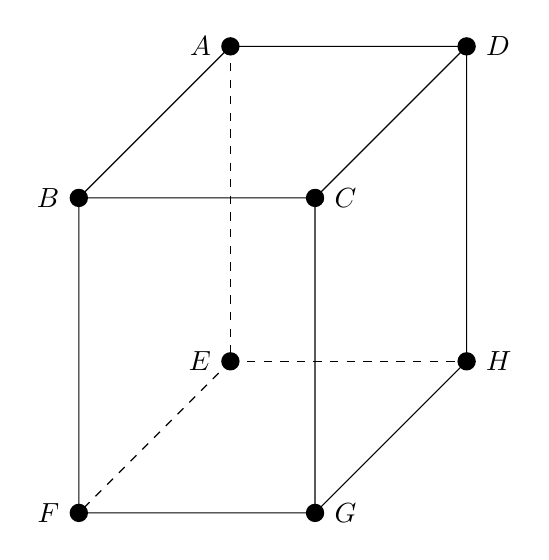
\begin{tikzpicture}[every edge quotes/.append style={auto, text=blue}]
				\pgfmathsetmacro{\cubex}{3}
				\pgfmathsetmacro{\cubey}{4}
				\pgfmathsetmacro{\cubez}{5}
				%%空間坐標中的CUBE 是以平面上的x軸 y軸再去擴充出深度z軸 z 往前為正,向後為負
				\coordinate (A) at (0,0,0);
				\coordinate (B) at (0,0,\cubez);
				\coordinate (C) at (\cubex, 0, \cubez );
				\coordinate (D) at (\cubex,0,0);
				\coordinate (E) at (0, -\cubey, 0);
				\coordinate (F) at (0, -\cubey, \cubez);
				\coordinate (G) at (\cubex, -\cubey, \cubez);
				\coordinate (H) at (\cubex, -\cubey, 0); 
				\draw [draw=black, every edge/.append style={draw=black, dashed}]
				(A) -- (B) --(C) --(D) -- cycle
				(C) -- (G) -- (H) -- (D) --cycle
				(B) -- (F) -- (G) -- (C) --cycle 
				(A) edge (E) 
				(E) edge (H)
				(E) edge (F);
				
				\foreach \v/\u/\t in 
				{A/180/$A$,
					B/180/$B$,
					C/0/$C$,
					D/0/$D$,
					E/180/$E$,
					F/180/$F$,
					G/0/$G$,
					H/0/$H$
				}
				{
					\draw[ultra thick,fill] (\v) circle (2.5pt);
					\node[label=\u:\t] at (\v){};
				};     
				\end{tikzpicture}
			\end{RightSidePic}
        \end{QBODY}
        \begin{QFROMS}
        \end{QFROMS}
        \begin{QTAGS}\QTAG{B4C1空間向量}\end{QTAGS}
        \begin{QANS}
            $\dfrac{4}{3}$
        \end{QANS}
        \begin{QSOLLIST}
			\begin{QSOL}
				\begin{LeftSide}[8cm]
					直角坐標坐標作法:\\
					\begin{QSTEPS}
						\QSTEP{ 令 $A(0,0,0), B(u,0,0), D(0,v,0), E(0,0,w) $}
						\QSTEP{ 由圖形可以知道平面$BDG$ 不會通過原點$A$,\\
							且與$x$, $y$, $z$ 軸皆有交點,且已知原平面過$B$, $D$ ,\\
							已有$x,y$ 截距,分別為 $u,v$\\
							可以假設 $E_{BDG}: \frac{x}{u} + \frac{y}{v} + \frac{z}{t} = 1$\\
							該平面通過$G(u,v,w)$ 代入可得:\\
							$1+1+\frac{w}{t}=1 \Rightarrow t= -w$\\
							$ \Rightarrow E_{BDG}: \frac{x}{u} + \frac{y}{v} + \frac{z}{-w} = 1 $
						}
						\QSTEP{ 由 $\lvec{AP} = \frac{1}{3} \lvec{AB} + 2 \lvec{AD} + a \lvec{AE} $\\
							可得點 $P$坐標為$ (\frac{1}{3} u, 2v, aw)$ \\
							且 $P$ 為平面 $BDG$ 上一點,\\
							代入滿足$E_{BDG}$ $\Rightarrow \frac{\frac{1}{3} u }{u}+\frac{2v}{v} + \frac{aw}{-w} = 1$ $\Rightarrow$\\
							 可解得 $a=\frac{4}{3}$ }
					\end{QSTEPS}
				\end{LeftSide}
				\begin{RightSidePic}
				   \begin{tikzpicture}
				   \pgfmathsetmacro{\cubex}{3}
				   \pgfmathsetmacro{\cubey}{4}
				   \pgfmathsetmacro{\cubez}{5}
				   %%空間坐標中的CUBE 是以平面上的x軸 y軸再去擴充出深度z軸 z 往前為正,向後為負
				   \coordinate (A) at (0,0,0);
				   \coordinate (B) at (0,0,\cubez);
				   
				   \coordinate (Bout) at (0,0,1.5*\cubez);
				   
				   \coordinate (C) at (\cubex, 0, \cubez );
				   \coordinate (D) at (\cubex,0,0);
				   
				   \coordinate (Dout) at (1.5*\cubex, 0, 0);
				   
				   \coordinate (E) at (0, -\cubey, 0);
				   
				   \coordinate (Eout) at (0, -\cubey *1.8, 0) ;
				   
				   \coordinate (F) at (0, -\cubey, \cubez);
				   \coordinate (G) at (\cubex, -\cubey, \cubez);
				   \coordinate (H) at (\cubex, -\cubey, 0); 
				   
				   \draw [draw=black, every edge/.append style={draw=black, dashed}]
				   (A) -- (B) --(C) --(D) -- cycle
				   (C) -- (G) -- (H) -- (D) --cycle
				   (B) -- (F) -- (G) -- (C) --cycle 
				   (A) edge (E) 
				   (E) edge (H)
				   (E) edge (F);
				   
				   \draw [fill=lightgray, opacity=0.5] (B)--(G)--(D) -- cycle;
				   
				   \draw[-{Stealth[scale=1.3,angle'=45]}, ultra thick] (A) -- (Dout) node[right] {$y$};
				   \draw[-{Stealth[scale=1.3,angle'=45]}, ultra thick] (A) -- (Bout) node[below] {$x$};
				   \draw[-{Stealth[scale=1.3,angle'=45]}, ultra thick] (A) -- (Eout) node[below] {$z$};
				   \foreach \v/\u/\t in 
				   {C/right/$C$,
					   F/left/$F$,
					   H/right/$H$
					}
					{
						\draw[ultra thick,fill] (\v) circle (2.5pt);
						\node[\u] at (\v){\t};
					};     
					\draw[ultra thick,fill] (A) circle (2.5pt);
					\draw[ultra thick,fill] (B) circle (2.5pt);
					\draw[ultra thick,fill] (D) circle (2.5pt);
					\draw[ultra thick,fill] (E) circle (2.5pt);
					\draw[ultra thick,fill] (G) circle (2.5pt);
					
					\node[above] at (A){$A(0,0,0)$};
					\node[label={[shift={(-1,0)}]$B(u,0,0)$} ] at (B) {};
					\node[above] at (D){$D(0,v,0)$};
					\node[right] at (G){$G(u,v,w)$};
					\node[label={[shift={(-1,0)}]$E(0,0,w)$}] at (E){};
					
					\end{tikzpicture}
				\end{RightSidePic}
			\end{QSOL}
        
			\begin{QSOL}
			   \begin{LeftSide}[8cm]
			   採用向量坐標\\

				   \begin{QSTEPS}
					   \QSTEP{令 $\lvec{AB}, \lvec{AD}, \lvec{AE}$ 為基底向量,$A$ 為坐標原點 \\
						   可知:$B(1,0,0),D(0,1,0), G(1,1,1) , P(\frac{1}{3}, 2 , a)$ }
						\QSTEP{先計算 $E_{BDG}:$\\
							找法向量:$\lvec{BD} = (-1,1,0), \lvec{BG} = (0,1,1) $\\
							$\Rightarrow \lvec{BD}\times \lvec{BG} = (1,1,-1) $ \\
							取法向量為 $\lvec{n} =(1,1,-1)$\\
							找點:$G(1,1,1)$ \\
							$\Rightarrow E_{BDG}: x+y-z=1$
						}
						\QSTEP{$P\in E_{BDG}$,$P$ 點坐標代入可得\\ $\frac{1}{3} + 2-a =1 \Rightarrow a = \frac{4}{3}$ }
					\end{QSTEPS}
				\end{LeftSide}
			   \begin{RightSidePic}
				   \begin{tikzpicture}
				   \pgfmathsetmacro{\cubex}{3}
				   \pgfmathsetmacro{\cubey}{4}
				   \pgfmathsetmacro{\cubez}{5}
				   %%空間坐標中的CUBE 是以平面上的x軸 y軸再去擴充出深度z軸 z 往前為正,向後為負
				   \coordinate (A) at (0,0,0);
				   \coordinate (B) at (0,0,\cubez);
				   
				   \coordinate (Bout) at (0,0,1.5*\cubez);
				   
				   \coordinate (C) at (\cubex, 0, \cubez );
				   \coordinate (D) at (\cubex,0,0);
				   
				   \coordinate (Dout) at (1.5*\cubex, 0, 0);
				   
				   \coordinate (E) at (0, -\cubey, 0);
				   
				   \coordinate (Eout) at (0, -\cubey *1.8, 0) ;
				   
				   \coordinate (F) at (0, -\cubey, \cubez);
				   \coordinate (G) at (\cubex, -\cubey, \cubez);
				   \coordinate (H) at (\cubex, -\cubey, 0); 
				   
				   \draw [draw=black, every edge/.append style={draw=black, dashed}]
				   (A) -- (B) --(C) --(D) -- cycle
				   (C) -- (G) -- (H) -- (D) --cycle
				   (B) -- (F) -- (G) -- (C) --cycle 
				   (A) edge (E) 
				   (E) edge (H)
				   (E) edge (F);
				   
				   \draw [fill=lightgray, opacity=0.5] (B)--(G)--(D) -- cycle;
				   
				   \draw[-{Stealth[scale=1.3,angle'=45]}, ultra thick] (A) -- (Dout) node[right] {$y$};
				   \draw[-{Stealth[scale=1.3,angle'=45]}, ultra thick] (A) -- (Bout) node[below] {$x$};
				   \draw[-{Stealth[scale=1.3,angle'=45]}, ultra thick] (A) -- (Eout) node[below] {$z$};
				   \foreach \v/\u/\t in 
				   {C/right/$C$,
					   F/left/$F$,
					   H/right/$H$
					}
					{
						\draw[ultra thick,fill] (\v) circle (2.5pt);
						\node[\u] at (\v){\t};
					};     
					\draw[ultra thick,fill] (A) circle (2.5pt);
					\draw[ultra thick,fill] (B) circle (2.5pt);
					\draw[ultra thick,fill] (D) circle (2.5pt);
					\draw[ultra thick,fill] (E) circle (2.5pt);
					\draw[ultra thick,fill] (G) circle (2.5pt);
					
					\node[above] at (A){$A(0,0,0)$};
					\node[label={[shift={(-1,0)}]$B(1,0,0)$} ] at (B) {};
					\node[above] at (D){$D(0,1,0)$};
					\node[right] at (G){$G(1,1,1)$};
					\node[label={[shift={(-1,0)}]$E(0,0,1)$}] at (E){};
					
					\end{tikzpicture}
				\end{RightSidePic}
			\end{QSOL}
        
		   \begin{QSOL}
			   採用共面定理:\\
			   $\lvec{AP} 
			   = \frac{1}{3}\lvec{AB} + 2 \lvec{AD} + a(\lvec{AG} - \lvec {AB} -\lvec{AD} ) 
			   = (\frac{1}{3} - a) \lvec{AB} + (2-a) \lvec{AD} + a \lvec{AG} $
			   
			   根據共面定理可得:$(\frac{1}{3} - a) + (2-a) +a = 1 \Rightarrow a = \frac{4}{3} $\\
			   \vspace{1.5cm}\\
			   \psset{cornersize=absolute,linearc=.2\baselineskip} 
			   \psframebox[framesep=15pt]
			   {		
				   \begin{minipage}[c]{14cm}
					   共面定理:在空間坐標中,$O$ 與 $A,B,C$ 不共面, 有一點 $P$ \\
					   使得 $\lvec{OP} = \alpha \lvec{OA} +\beta \lvec{OB} +\gamma \lvec{OC} $ \\
					   若 $A,B,C,P$ 共面 ,則$\alpha+\beta+\gamma = 1$
					\end{minipage}
				}
			\end{QSOL}
        \end{QSOLLIST}
        \begin{QEMPTYSPACE}
        \end{QEMPTYSPACE}
    \end{QUESTION}
\end{QUESTIONS}
